
%(BEGIN_QUESTION)
% Copyright 2008, Tony R. Kuphaldt, released under the Creative Commons Attribution License (v 1.0)
% This means you may do almost anything with this work of mine, so long as you give me proper credit

A very useful principle in physics is the {\it Ideal Gas Law}, so called because it relates pressure, volume, molecular quantity, and temperature of an ideal gas together in one neat mathematical expression:

$$PV = nRT$$

\noindent
Where,

$P$ = Absolute pressure (atmospheres)

$V$ = Volume (liters)

$n$ = Gas quantity (moles)

$R$ = Universal gas constant (0.0821 L $\cdot$ atm / mol $\cdot$ K)

$T$ = Absolute temperature (K)

\vskip 10pt

Apply this law to the scenario of a gas-filled cylinder and movable piston:

$$\includegraphics[width=15.5cm]{i02923x01.eps}$$

In particular, sketch how the gas pressure inside the cylinder relates to changes in cylinder volume caused by piston movement, assuming no change in gas temperature or leakage of gas molecules from the cylinder:

$$\includegraphics[width=15.5cm]{i02923x02.eps}$$

\vfil 

\underbar{file i02923}
\eject
%(END_QUESTION)





%(BEGIN_ANSWER)

$$\includegraphics[width=15.5cm]{i02923x03.eps}$$

Note that the function is a curve and not a straight line!  In essence, the function plotted is this:

$$P = {k \over V}$$

Where $k$ is a constant equal to $nRT$.
 
%(END_ANSWER)





%(BEGIN_NOTES)

%INDEX% Physics, static fluids: ideal gas law

%(END_NOTES)


